\documentclass[conference]{IEEEtran}
\IEEEoverridecommandlockouts
% The preceding line is only needed to identify funding in the first footnote. If that is unneeded, please comment it out.
\usepackage{cite}
\usepackage{amsmath,amssymb,amsfonts}
\usepackage{algorithmic}
\usepackage{graphicx}
\usepackage{textcomp}
\usepackage{xcolor}
\usepackage{booktabs}
\usepackage{multirow}
\usepackage{tikz}
\usepackage{pgfplots}
\pgfplotsset{compat=1.18}
\def\BibTeX{{\rm B\kern-.05em{\sc i\kern-.025em b}\kern-.08em
    T\kern-.1667em\lower.7ex\hbox{E}\kern-.125emX}}
\begin{document}

\title{Blockchain based Anonymous Authentication Framework for Healthcare IoT\\

}

\author{\IEEEauthorblockN{1\textsuperscript{st} Smt. Ch Vijayalakshmi}
\IEEEauthorblockA{\textit{Department of Computer Science and Engineering} \\
\textit{Chaitanya Bharathi Institute of Technology}\\
Hyderabad, Telangana, India \\
[vijayalakshmich\_cse@cbit.ac.in](mailto:vijayalakshmich\_cse@cbit.ac.in)}
\and
\IEEEauthorblockN{2\textsuperscript{nd} M. Maruthi kalyan Reddy}
\IEEEauthorblockA{\textit{Department of Computer Science and Engineering} \\
\textit{Chaitanya Bharathi Institute of Technology}\\
Hyderabad, Telangana, India \\
[kalyanr2200@gmail.com](mailto:kalyanr2200@gmail.com)}
\and
\IEEEauthorblockN{3\textsuperscript{rd} R. Sai Charan}
\IEEEauthorblockA{\textit{Department of Computer Science and Engineering} \\
\textit{Chaitanya Bharathi Institute of Technology}\\
Hyderabad, Telangana, India \\
[ramunisaicharan@gmail.com](mailto:ramunisaicharan@gmail.com)}
}

\maketitle

\begin{abstract}
Healthcare Internet of Things (IoT) connects patients, medical devices, and healthcare
providers to enable real-time monitoring and efficient healthcare services. However, these
systems face critical challenges in secure authentication, as sensitive medical data is highly
vulnerable to forgery, malicious key generation, and privacy breaches. Ensuring anonymity is
equally essential to prevent identity leakage, which may compromise patient confidentiality
and trust. Existing certificateless signature (CLS) schemes provide a foundation for
lightweight authentication with anonymity, integrity, and resistance to replay. Nevertheless,
these schemes remain limited in handling malicious key generation and limited flexibility in
dynamic healthcare environments. To address these issues, this work proposes an enhanced
certificateless signature (CLS) scheme that achieves anonymity while resisting malicious key
generation, secret key exposure, and signature forgery. The scheme ensures data integrity
through a hybrid framework that supports both blockchain-based and non-blockchain
deployment, providing flexibility for different healthcare environments. In addition, the
proposed approach can be extended with revocation mechanisms to eliminate malicious users
and attackers, thereby enhancing long-term system resilience.

\end{abstract}

\begin{IEEEkeywords}
Healthcare Internet of Things (IoT), certificateless signature (CLS),
authentication, anonymity, data integrity, blockchain, security, revocation.
\end{IEEEkeywords}

\section{Introduction}

The swift expansion of IoT into the realm of healthcare has sparked a revolutionary shift in how healthcare services are provided and received. The Healthcare Industrial Internet of Things (Healthcare IIoT) revolutionizes traditional care by virtue of its capabilities to perceive everything, analyze intelligently, and operate independently of human interference \cite{ref1,ref2}. In healthcare IIoT, researchers attach tiny biosensors, including pulse oximeters, ECG patches, continuous glucose monitorers, and blood pressure cuffs, directly onto patient's body to sense the patient's physiological parameters, which include the level of blood oxygen saturation, heart rate, respiration rate, and body temperature \cite{ref3}. Due to the huge volume of data generated by these sensors, as well as the limited processing capabilities of the wearable devices themselves, medical researchers must outsource EHR data to cloud-based and distributed ledgers for persistent storing and analyzing, not to mention inter-hospital EHR data exchange \cite{ref4,ref5}.
In general, the open and heterogeneous environment of wireless communication in Healthcare IIoT subjects the EHR data to multiple kinds of attacks. Some attacks that adversaries could launch against the EHR data include forgery attacks, man-in-the-middle attacks, replay attacks, and eavesdropping attacks\cite{ref6}. The disclosure and unauthorized modification of sensitive health information not only damages patient privacy but can directly threaten patient safety by leading to erroneous clinical decisions---incorrect drug dosages, missed diagnoses, or falsified laboratory results---thereby deteriorating the integrity of the doctor-patient relationship \cite{ref7}. Moreover, in smart healthcare systems, both medical personnel and patients frequently access the system to retrieve or update health-related information; unauthorized access by adversaries may lead to catastrophic consequences including identity theft, data leakage\cite{ref8}, and the misuse of personal health data . Therefore, ensuring the authenticity, integrity, confidentiality, and availability of EHR data, while simultaneously establishing a secure and lightweight authentication mechanism, has become a critical and urgent research imperative.

Digital signatures serve as a fundamental cryptographic tool to provide identity authentication, data integrity verification, and non-repudiation in electronic data transmission \cite{ref9}. In the context of Healthcare IIoT, a robust digital signature framework must satisfy several stringent yet often conflicting requirements: (i) computational efficiency suitable for resource-constrained wearable devices with limited battery life and processing power; (ii) minimal communication overhead to accommodate bandwidth-limited sensor networks; (iii) strong privacy guarantees to comply with regulatory frameworks such as HIPAA and GDPR; and (iv) mutual authentication between communicating parties to prevent impersonation and unauthorized EHR access \cite{ref10,ref11}. Critically, we observe that not all healthcare interactions demand the same level of infrastructure. A routine telemedicine consultation between a patient and a doctor requires fast, lightweight mutual authentication---but does not necessarily warrant the overhead of a full blockchain transaction. Conversely, uploading an official EHR for cross-hospital sharing or regulatory auditing mandates immutable on-chain storage with verifiable provenance. This fundamental asymmetry in operational requirements motivates the hybrid architecture proposed in this work.


\subsection{Motivation}

The construction of an efficient and reliable authentication scheme for Healthcare IIoT requires rigorous attention to the cryptographic foundation as well as the system deployment architecture. The traditional PKI-based signature mechanisms face unaffordable certificate management complexity when scaling up the number of involved parties to cover patients, doctors, nurses, and sensor nodes. In addition, the IBC approach dispenses with certificates but suffers from the key escrow issue. The key generation center (KGC) holds all the secret keys, which enables any adversary controlling the KGC to forge signatures of arbitrary users. Such an attack is completely intolerable in clinical practice \cite{ref12}. On the other hand, CL-PKC solves both issues by distributing the private key among the KGC and the user. However, most existing CLS approaches do not satisfy Girault's Level-3 security requirements \cite{ref13}.

Apart from the cryptographic foundation, real-world deployment on energy-limited clinical wearables entails strict resource limitations. The most costly elliptic curve cryptographic primitive is the scalar multiplication ($T_{Mu}$). Most provably secure CLS frameworks demand at least one scalar multiplication for generating a digital signature. Such a requirement consumes significant battery power and creates unacceptable latency, making it impractical for real-time EHR transfer applications like ECG patches and pulse oximeters \cite{ref14}. Furthermore, current CLS schemes with formal security proofs mandate four or more distinct cryptographic hash function invocations per signature, compounding the computational burden on constrained processors \cite{ref15}.

Authentication itself also faces many obstacles. Currently, a majority of healthcare systems adopt biometric fuzzy extractors that generate cryptographic keys from noisy biometric signals \cite{ref16}. Although biometric fuzzy extraction offers an intriguing prospect, the scheme involves non-trivial False Rejection Rates (FRR) when applied to physiological stress factors common in clinical scenarios such as trembling hands, sweating, and skin abrasions, resulting in legitimate users being denied access in emergency situations. Hence, a credential-based multi-factor authentication solution becomes indispensable. In addition, most CLS-based authentication protocols offer a one-size-fits-all authentication mechanism without regard for user identity at the cryptographic level \cite{ref17}. In contrast, patients and doctors in healthcare settings have completely different roles.

Most importantly, the current blockchain-based healthcare authentication systems exhibit inflexibility in terms of architectural design, requiring either full blockchain overhead for each transaction or no blockchain at all, which compromises accountability. Yet, there exists no patient-selectable hybrid architecture, enabling participants to decide whether off-chain authentication and/or EHR storage using blockchain technology is necessary.

\subsection{Our Contributions}

In order to overcome the above-mentioned obstacles, we introduce a \textit{Hybrid Blockchain-Based Certificateless Conditional Anonymous Authentication Framework for Secure EHR Sharing in Healthcare IIoT}. This framework is distinctively structured on a dual-mode architecture that enables participants to select the appropriate security-performance trade-off for each clinical interaction. The principal contributions of this work are summarized as follows.

\begin{itemize}
\item \textbf{Zero-$T_{Mu}$ Certificateless Signature Scheme:} We propose a pairing-free CLS scheme with no elliptic curve scalar multiplication operations in the online signing stage by leveraging pre-computed Secret Identifiers. The proposed CLA-based hash function significantly decreases the number of hashing operations to two, resulting in a very lightweight signature generation cost of $0\,T_{Mu} + 2\,T_{ha} + 6\,T_{mu}$.

\item \textbf{Dual-Mode Hybrid Architecture:} We construct a user-selective approach that allows two different modes of operation: a Lightweight Mode for peer-to-peer off-chain mutual authentication during telemedicine consultations, and a Blockchain-Anchored Mode for immutable on-chain EHR entries and cross-hospital EHR exchange.

\item \textbf{Dual-Chain Blockchain with Chameleon Revocation:} For the on-chain mode, we implement a dual-chain architecture consisting of a Historical Verification Chain (HVC) chain for verifying EHR entries and an Evidence Revocation Chain (ERC) that employs Chameleon Hashing technique to selectively revoke EHR credentials without breaking the blockchain structure.


\item \textbf{Role-Aware Multifactor Mutual Authentication:} We incorporate a deterministic multifactor verification mechanism with knowledge and possession tokens in lieu of biometric fuzzy extractors. The model inherently includes the roles of the actors (PATIENT/DOCTOR) within the pseudonyms to prevent cross-role impersonation of EHRs.
\item \textbf{Performance Analysis:} Thorough theoretical cost analysis and simulation on a testbed show the superior latency, throughput, and communication overhead of our authentication framework relative to current authentication schemes for health care.

\end{itemize}

The remainder of this paper is structured as follows: Section II reviews related literature. Section III outlines the mathematical preliminaries. Section IV describes the system and threat models. Section V details the proposed certificateless signature and dual-mode blockchain architectures. Section VI provides the formal security proofs, while Section VII details the mutual authentication protocol. Section VIII evaluates performance, followed by concluding remarks in Section IX.


\section{Related Works}

This section critically reviews the relevant literature along two converging research avenues: certificateless signature schemes for IoT systems and blockchain-enabled authentication methods for medical data exchange. We then provide an analysis that contrasts our hybrid approach with existing literature.

\subsection{Certificateless Signature Schemes for IoT}

Certificateless public key cryptography (CL-PKC), proposed by Al-Riyami and Paterson \cite{ref18}, addresses the disadvantages of traditional PKI, which require costly certificate management, and those of IBC, which suffer from a key escrow problem. The full private key of each user is generated based on the KGC-issued partial private key and a personal secret chosen by the user, guaranteeing that no forgery can be carried out by the KGC alone. Since CL-PKC was first proposed, many CLS schemes have been put forward, with a clear evolutionary trend from pairing-based to pairing-free constructions.

Some early pairing-based CLS schemes \cite{ref19,ref20} attained their security guarantee under the Bilinear Diffie-Hellman assumption, but the computation cost associated with their bilinear pairings became excessive. Hence, the idea of achieving CLS without using bilinear pairings through ECC proved to be more attractive. Yet, devising such a pairing-free CLS scheme is extremely difficult and leads to an endless loop of cryptanalysis and improvement.

One of the first attempts towards constructing a pairing-free CLS scheme for IIoT applications is made by Karati et al. \cite{ref20}, which claimed to provide existential unforgeability. Soon afterward, another pairing-free CLS scheme was developed by Jia et al. \cite{ref21} to claim its security. Later on, Du et al. \cite{ref23} and Xiang et al. \cite{ref24} pointed out that Jia et al.'s scheme is susceptible to Type-I (external) adversary forgery attacks, and hence, devised better schemes accordingly. In turn, Ma et al. \cite{ref22} successfully launched forgery attacks on Du et al.'s and Xiang et al.'s schemes and showed their insecurity against forgery.

Thumbur et al. \cite{ref11} introduced an efficient CLS scheme specifically for resource-constrained environments. Xu et al. \cite{ref21} subsequently proved that Thumbur et al.'s scheme could be trivially forged by a Type-I adversary. Wang et al. \cite{ref1} then demonstrated that Xu et al.'s own repair was still vulnerable to replay attacks and KGC compromise, and proposed a Blockchain-Based Certificateless Conditional Anonymous Authentication (BCCA) scheme with precomputed key materials and batch verification. However, Shim \cite{ref23} later exposed a critical flaw in Wang et al.'s signing algorithm: the omission of a per-session random nonce allowed an attacker to recover a user's complete private key from merely two intercepted signatures.

Addressing the persistent insecurity of pairing-free CLS schemes against malicious KGCs, Qiao et al. \cite{ref24} formally demonstrated that virtually all preceding pairing-free CLS constructions fail to achieve Girault Level-3 security—the highest trust level, wherein even a fully compromised KGC cannot forge valid signatures. Qiao et al. proposed a provably secure CLS scheme with anonymity that achieves Level-3 under the hardness of the discrete logarithm problem (DLP) in the random oracle model. Despite its strong security guarantees, the scheme requires one online elliptic curve scalar multiplication ($T_{Mu}$) and four distinct hash invocations per signature—overhead that remains prohibitive for battery-powered clinical sensors transmitting continuous physiological data streams.

\begin{table*}[htbp]
\centering
\caption{Feature Comparison of Related Authentication Schemes}
\label{tab:comparison}
\renewcommand{\arraystretch}{1.2}
\setlength{\tabcolsep}{4pt}
\begin{tabular}{|l|c|c|c|c|c|c|c|c|}
\hline
\textbf{Feature} & \textbf{He \cite{ref27}} & \textbf{Ma \cite{ref22}} & \textbf{Wang \cite{ref1}} & \textbf{Qiao \cite{ref24}} & \textbf{Tang \cite{ref25}} & \textbf{Meher \cite{ref28}} & \textbf{Soni \cite{ref26}} & \textbf{Ours} \\
\hline
Healthcare Focus & $\checkmark$ & $\times$ & $\checkmark$ & $\times$ & $\checkmark$ & $\checkmark$ & $\checkmark$ & $\checkmark$ \\
\hline
Certificateless \& Pairing-Free & $\times$ & $\checkmark$ & $\checkmark$ & $\checkmark$ & $\times$ & $\times$ & $\times$ & $\checkmark$ \\
\hline
Provable Security Guarantee & $\checkmark$ & $\checkmark$ & $\times$ & $\checkmark$ & $\checkmark$ & $\checkmark$ & $\checkmark$ & $\checkmark$ \\
\hline
Conditional Anonymity & $\checkmark$ & $\checkmark$ & $\checkmark$ & $\checkmark$ & $\checkmark$ & $\checkmark$ & $\times$ & $\checkmark$ \\
\hline
Mutual Authentication & $\checkmark$ & $\checkmark$ & $\times$ & $\times$ & $\checkmark$ & $\checkmark$ & $\checkmark$ & $\checkmark$ \\
\hline
Blockchain Integration & $\times$ & $\times$ & $\checkmark$ & $\times$ & $\checkmark$ & $\times$ & $\checkmark$ & $\checkmark$ \\
\hline
Auditable Revocation Mechanism & $\times$ & $\times$ & $\checkmark$ & $\times$ & $\times$ & $\times$ & $\times$ & $\checkmark$ \\
\hline
Girault Level-3 Trust & $\times$ & $\times$ & $\times$ & $\checkmark$ & $\times$ & $\times$ & $\times$ & $\checkmark$ \\
\hline
Zero Online $T_{Mu}$ Overhead & $\times$ & $\times$ & $\times$ & $\times$ & $\times$ & $\times$ & $\times$ & $\checkmark$ \\
\hline
Hybrid Mode (On/Off-Chain) & $\times$ & $\times$ & $\times$ & $\times$ & $\times$ & $\times$ & $\times$ & $\checkmark$ \\
\hline
\end{tabular}
\end{table*}


\subsection{Blockchain-Assisted Healthcare Authentication}

The healthcare ecosystem has widely implemented blockchain technology to offer immutable audit trails and ensure trust between multiple parties by enabling data provenance. Tang et al. \cite{ref25} provided a robust authentication system based on blockchains and smart contracts for EHR applications, although they didn't utilize certificateless cryptography and therefore carried over the drawbacks related to certificate management of PKI schemes. Another example is that of Yazdinejad et al., who designed a decentralized authentication system for distributed hospital network environments \cite{ref25}, even though their protocol was neither formally verified nor satisfied the condition of anonymity.

Wireless body area networks (WBANs) constitute one of the most significant parts of the Healthcare IIoT infrastructure, where various authentication schemes have been developed. For instance, He et al. \cite{ref27} introduced a protocol for anonymous authentication in WBANs and proved its security properties; however, such protocol uses bilinear pairing calculations. Xiong introduced a more resource-friendly anonymous certificateless remote authentication scheme for WBANs \cite{ref29}; at the same time, Xiong and Qin revealed weaknesses in large-scale deployment of this protocol . Next, Liu et al. \cite{ref26} enhanced existing two-layer authentication protocol, yet still without blockchain functionality or mutual authentication support. Recently, Meher et al. \cite{ref28} proposed an anonymous mutual authentication scheme for WBANs based on DLP, ECDLP and bilinear pairing operations. Meher et al. achieved the strong security guarantees and mutual authentication, but's hybrid approach inherently retains the computational cost of pairings, limiting its applicability on ultra-constrained clinical sensors.

The research work by Soni et al. \cite{ref26} proposed Blockchain-Based User Authentication and Data-Sharing (BC-UADS) framework for healthcare industries that used consortium blockchain model and the Proof-of-Reputation consensus mechanism. The framework offers support for mutual authentication and multi-hospital EHR sharing but did not use certificateless cryptography and, therefore, cannot withstand certificate attack. Zhu et al. \cite{ref2} created certificateless redactable signature scheme with batch verification for Healthcare IoT and integrated the concept of privacy-preserving data sharing and efficient verification of multi-signature. This scheme does not offer conditional anonymity and role-based access control.

The most important architectural issue inherent almost in all the present-day blockchain healthcare frameworks is their rigidity and single-mode approach; namely, the traffic of authentication is inevitably passed through the blockchain regardless of the particular case. Wang et al. \cite{ref1} provided a partial solution to the problem of flexible revocation through introduction of a dual chain system that allowed separating historical records for verification and evidence about revocation with the help of chameleon hashing. Unfortunately, their blockchain still requires passing everything through on the blockchain without providing any flexibility.


\subsection{Literature Summary and Comparison}

To synthesize the current state of research across both certificateless cryptography and blockchain-based healthcare authentication, Table~\ref{tab:comparison} presents a feature-level comparison of the strongest representative schemes against our proposed framework. By selecting highly competitive recent protocols—many of which achieve provable security, mutual authentication, and conditional anonymity—the comparison reveals that while individual works excel in specific domains, no existing scheme simultaneously bridges all gaps. Our proposed framework is unique in aggregating pairing-free certificateless design, Girault Level-3 security, zero online scalar multiplications, and an auditable blockchain-based revocation system into a unified, patient-selectable hybrid architecture.

Cryptographically, our scheme builds upon the Level-3 security foundation established by Qiao et al.~\cite{ref24} but substantially reduces the signing overhead through precomputed Secret Identifier (SID) arrays and a novel Carry Look-Ahead (CLA)-based hash derivation. This design eliminates all online scalar multiplications and reduces hash invocations from four to two per signature. Architecturally, we inherit the dual-chain chameleon hash revocation model pioneered by Wang et al.~\cite{ref1} but critically decouple the authentication layer from the blockchain layer.  This breakthrough drops the online signing cost from $1,T_{Mu} + 4,T_{ha}$ down to $0,T_{Mu} + 2,T_{ha}$, making it significantly lighter than Qiao et al.'s model. This decoupling enables a patient-selectable hybrid operational mode: a \textit{Lightweight Mode} for direct peer-to-peer mutual authentication during routine telemedicine sessions, and a \textit{Blockchain-Anchored Mode} for immutable, auditable EHR storage. To the best of our knowledge, no prior work offers this dual-mode flexibility within a unified certificateless framework.

\section{Preliminaries}

This section introduces the mathematical foundations, cryptographic definitions, and the formal security model underlying the proposed hybrid certificateless authentication framework. Table~\ref{tab:notation} summarizes the principal notation used throughout the remainder of this paper.

\begin{table}[htbp]
\centering
\caption{Notation Summary}
\label{tab:notation}
\renewcommand{\arraystretch}{1.2}
\setlength{\tabcolsep}{6pt}
\begin{tabular}{|c|p{4.5cm}|}
\hline
\textbf{Symbol} & \textbf{Description} \\
\hline
$\kappa$ & Security parameter \\
\hline
$E(\mathbb{F}_q)$ & Elliptic curve over the finite field $\mathbb{F}_q$ \\
\hline
$G$ & Additive cyclic group of prime order $q$ on $E(\mathbb{F}_q)$ \\
\hline
$P$ & Generator of $G$ \\
\hline
$\mathcal{O}$ & Point at infinity (identity element of $G$) \\
\hline
$s$ & System master secret key \\
\hline
$P_{pub} = sP$ & System master public key \\
\hline
$P_{pub1}, P_{pub2}$ & CLA-derived domain-separated public keys (blockchain mode) \\
\hline
$RID_i$ & Real identity of user $U_i$ \\
\hline
$ID_i$ & Pseudonym (anonymous identity) of $U_i$ \\
\hline
$x_i$ & User's self-chosen secret value \\
\hline
$upk_i = x_i P$ & User's public key \\
\hline
$d_i$ (or $psk_i$) & Partial private key issued by KGC/HA \\
\hline
$gpk_i = k_i P$ & Partial public key corresponding to $psk_i$ \\
\hline
$SK_i = (x_i, psk_i)$ & User's full private key \\
\hline
$PK_i = (upk_i, gpk_i)$ & User's full public key \\
\hline
$SID_{i,k}$ & $k$-th precomputed secret key from the SID set \\
\hline
$KID_{i,k} = SID_{i,k} \cdot P$ & $k$-th precomputed public key from the KID set \\
\hline
$\psi$ & CLA carry-in value, $\psi = x\text{-coord}(KID_k) \bmod q$ \\
\hline
$H_0, H_1, H_2, H_3$ & Cryptographic hash functions (modeled as random oracles) \\
\hline
$\oplus$ & Bitwise XOR operation \\
\hline
$T_{Mu}$ & Time cost of one EC scalar multiplication \\
\hline
$T_{Add}$ & Time cost of one EC point addition \\
\hline
$T_{ha}$ & Time cost of one general hash operation \\
\hline
$T_{mu}$ & Time cost of one modular multiplication \\
\hline
$\Delta T$ & Maximum allowable timestamp deviation (freshness window) \\
\hline
\end{tabular}
\end{table}

\subsection{Elliptic Curve Cryptography}

Let $q$ be a large prime and $\mathbb{F}_q$ a finite field. A non-singular elliptic curve over $\mathbb{F}_q$ is defined as:
\begin{equation}
E(\mathbb{F}_q) : y^2 = x^3 + ax + b \pmod{q}
\end{equation}
where $a, b \in \mathbb{F}_q$ and $4a^3 + 27b^2 \not\equiv 0 \pmod{q}$. The set of all points on $E(\mathbb{F}_q)$ together with the point at infinity $\mathcal{O}$ forms an additive cyclic group $G$ with generator $P$ and prime order $q$. For any point $Q \in G$ and scalar $k \in \mathbb{Z}_q^*$, the scalar multiplication $Q = kP$ is efficiently computable, but its inverse—recovering $k$ given $Q$ and $P$—is computationally intractable.

\subsection{Hardness Assumptions}

\textbf{Definition 1 (Discrete Logarithm Problem — DLP).} Given the additive cyclic group $G$ of prime order $q$ with generator $P$, and a random point $Q = aP$ where $a \in \mathbb{Z}_q^*$, the DLP is to compute $a$ from $(P, Q)$. The DL assumption states that for any probabilistic polynomial-time (PPT) adversary $\mathcal{A}$, the advantage
\begin{equation}
\text{Adv}^{DL}_{\mathcal{A}}(\kappa) = \Pr[\mathcal{A}(P, aP) = a]
\end{equation}
is negligible in $\kappa$.

\textbf{Definition 2 (Elliptic Curve Discrete Logarithm Problem — ECDLP).} Given a point $Q \in G$ and the generator $P$ of $G$, the ECDLP is to find $x \in \mathbb{Z}_q^*$ such that $Q = xP$. Finding such $x$ is computationally infeasible for appropriately chosen parameters~\cite{ref30}.

\textbf{Definition 3 (Elliptic Curve Computational Diffie--Hellman Problem — ECCDHP).} Given $(P, aP, bP) \in G$ for unknown $a, b \in \mathbb{Z}_q^*$, the ECCDHP is to compute $abP$. The ECCDH assumption states that no PPT adversary can solve this problem with non-negligible probability.

\textit{Remark:} The security of the proposed CLS scheme and mutual authentication protocol relies on the hardness of the DLP. The ECCDHP underpins the security of the Diffie--Hellman-based session key agreement in the mutual authentication phase.

\subsection{Girault's Security Levels for CL-PKC}

Girault~\cite{ref13} defined a hierarchy of trust levels for key generation centers (KGCs) in certificateless and certificate-based cryptographic schemes. Hu et al. subsequently extended this classification to the CLS setting:

\begin{itemize}
\item \textbf{Level 1:} The KGC possesses sufficient information to compute users' full private keys and can impersonate any user.
\item \textbf{Level 2:} The KGC does not know users' full private keys but can generate fraudulent partial keys that pass verification.
\item \textbf{Level 3:} The KGC cannot forge valid signatures even by fabricating partial private keys, as inconsistencies with user public keys are detectable.
\end{itemize}

\textit{Significance:} Level 3 provides the strongest trust guarantee: even a fully compromised Hospital Administrator (serving as the KGC) cannot forge a valid patient or doctor signature. The proposed scheme achieves Girault Level-3 by binding the partial private key $psk_i$ to the user's public key $upk_i$ within the hash computation
\begin{equation}
h_1 = H_1(ID_i, gpk_i, upk_i, P_{pub}, E_i)
\end{equation}
ensuring that any substitution by the KGC is publicly detectable.

\subsection{Chameleon Hash Function}

A Chameleon Hash function~\cite{ref43}, introduced by Krawczyk and Rabin, is a trapdoor collision-resistant hash function. It consists of the following algorithms:

\begin{itemize}
\item \textbf{Setup}$(\lambda)$: Outputs public parameters $pp$.
\item \textbf{KeyGen}$(pp)$: Outputs $(HK, ck)$, where $HK$ is the hash key and $ck$ is the trapdoor key.
\item \textbf{Hash}$(HK, m, \zeta)$: Outputs hash value $CH$.
\item \textbf{Verify}$(HK, m, \zeta, CH)$: Verifies correctness of $CH$.
\item \textbf{Forge}$(ck, m, \zeta, m')$: Computes $\zeta'$ such that
\begin{equation}
\text{Hash}(HK, m, \zeta) = \text{Hash}(HK, m', \zeta').
\end{equation}
\end{itemize}

\textit{Security Properties:}
\begin{itemize}
\item \textbf{Collision Resistance:} Without $ck$, finding collisions is infeasible.
\item \textbf{Trapdoor Collision:} With $ck$, controlled collisions are efficiently computable.
\end{itemize}

In our framework, the Hospital Administrator holds the trapdoor key to enable controlled modification of revocation evidence without altering blockchain integrity.

\subsection{Carry Look-Ahead (CLA) Adder — Algebraic Hash Derivation}

The Carry Look-Ahead (CLA) adder computes carry bits in parallel:
\begin{equation}
C_{i+1} = G_i + P_i \cdot C_i
\end{equation}
where $G_i = A_i \cdot B_i$ and $P_i = A_i \oplus B_i$.


 It achieves this through two fundamental Boolean logic components: the "generate" signal (which produces a carry independent of previous states) and the "propagate" signal (which passes a carry forward if one exists).

In conventional pairing-free certificateless signature schemes, executing multiple independent cryptographic hash functions per transaction incurs significant computational overhead, rendering them suboptimal for continuous transmission in resource-constrained IIoT devices. We innovatively repurpose the structural logic of the CLA—specifically its generate and propagate characteristics—and map it onto the finite field $\mathbb{Z}^*_q$.



\subsection{Forking Lemma}

The Forking Lemma~ is used to prove signature security in the Random Oracle Model.

\textbf{Lemma 1:} If a PPT adversary $\mathcal{A}$ produces a valid forgery with probability $\varepsilon$ after $Q_h$ hash queries, then a PPT algorithm can extract two forgeries with probability:
\begin{equation}
\varepsilon' \geq \left(1 - \frac{1}{e}\right)\frac{\varepsilon}{Q_h}.
\end{equation}

\textit{Application:} The lemma is applied to hash oracles $H_1$ and $H_2$ to extract two valid signatures, enabling reduction to the DLP and proving unforgeability.

\section{Methodology}

In this section, we present the complete construction of the proposed Hybrid Blockchain-Based Certificateless Conditional Anonymous Authentication Framework for Healthcare IIoT. The framework consists of a common construction shared by both operational modes, a Lightweight Mode for off-chain peer-to-peer authentication, and a Blockchain-Anchored Mode for on-chain EHR operations. Each mode shares the same registration, key generation, and login infrastructure, diverging only at the signature and authentication layers. The scheme supports user revocation and on-chain evidence modification.

\subsection{Common Construction}

This phase consists of the following polynomial-time algorithms that are executed during system initialization and user onboarding. Their outputs serve both operational modes.
\section{Proposed Framework}

In this section, we present the complete construction of the proposed Hybrid Blockchain-Based Certificateless Conditional Anonymous Authentication Framework for Healthcare IIoT. The framework consists of a common construction shared by both operational modes, a Lightweight Mode for off-chain peer-to-peer authentication, and a Blockchain-Anchored Mode for on-chain EHR operations. Each mode shares the same registration, key generation, and login infrastructure, diverging only at the signature and authentication layers. The scheme supports user revocation and on-chain evidence modification.

\subsection{Common Construction}

This phase consists of the following polynomial-time algorithms executed during system initialization and user onboarding. Their outputs serve both operational modes.

\textit{Setup:} In this phase, the Hospital Administrator (HA) generates the system public parameters based on a security parameter $\kappa$.

\begin{enumerate}
\item Given $\kappa$, HA selects an elliptic curve $E$ over a finite field $\mathbb{F}_q$, and an additive cyclic group $G$ of prime order $q$ with generator $P$.

\item HA randomly selects $s \in \mathbb{Z}_q^*$ as the master secret key and computes the system master public key $P_{pub} = sP$.

\item HA performs CLA-based public key splitting for the Blockchain-Anchored Mode. Let $P_x = x\text{-coordinate}(P) \bmod q$. HA computes $G_{cla} = (s \cdot P_x) \bmod q$ and $Prop = (s \oplus P_x) \bmod q$, and derives $s_1 = G_{cla}$ and $s_2 = (G_{cla} + Prop) \bmod q$, yielding $P_{pub1} = s_1 \cdot P$ and $P_{pub2} = s_2 \cdot P$.

\item HA generates a decryption key pair: private key $y \in \mathbb{Z}_q^*$ (assigned to authorized doctors) and public key $dpk = y \cdot P$.

\item HA defines cryptographic hash functions modeled as random oracles:
$H_0 : G \times \{0,1\}^* \rightarrow \{0,1\}^*$,
$H_1 : \{0,1\}^* \rightarrow \mathbb{Z}_q^*$,
$H_2 : \{0,1\}^* \rightarrow \mathbb{Z}_q^*$,
$H_3 : \{0,1\}^* \rightarrow \mathbb{Z}_q^*$.

\item HA publishes:
$params_L = \{E, G, q, P, P_{pub}, H_0, H_1, H_2\}$ for Lightweight Mode and
$params_B = \{E, G, q, P, P_{pub}, P_{pub1}, P_{pub2}, dpk, H_1, H_2, H_3\}$ for Blockchain Mode.
\end{enumerate}

\textit{Set-Secret-Value:} In this phase, a user $U_i$ (patient or doctor) registers with HA via a secure channel.

\begin{enumerate}
\item $U_i$ selects a random secret $x_i \in \mathbb{Z}_q^*$ and computes the public key $upk_i = x_i \cdot P$.

\item $U_i$ inputs real identity $RID_i$ and password $PW_i$, and computes $UPW_i = H_1(RID_i, PW_i)$.

\item $U_i$ provides deterministic credentials. For patients: Date of Birth ($DOB$), blood group, emergency contact, and security answer ($SA$). For doctors: Date of Birth ($DOB$), medical registration number, and security answer ($SA$). Then computes $\alpha_i = H_1(DOB_i, SA_i, OtherDetails_i)$.

\item $U_i$ sends registration data $Reg_i = (upk_i, RID_i, UPW_i, \alpha_i, Role_i)$ to HA via a secure channel, where $Role_i \in \{PATIENT, DOCTOR\}$.
\end{enumerate}

\noindent\textit{Extract-partial-private-key:} In this phase, HA generates the user's partial private key and pseudonymous identity.

\begin{enumerate}
\item HA verifies the legitimacy of $U_i$'s real identity and role via medical licenses or hospital enrollment records.

\item HA chooses a random number $d_i \in \mathbb{Z}_q^*$ and computes $E_i = d_i \cdot P$. The pseudonym generation branches based on the architecture mode:

\begin{itemize}
\item \textit{Lightweight Mode:} $ID_i = RID_i \oplus H_0(s \cdot E_i, V_t)$, where $V_t$ is the validity period.

\item \textit{Blockchain-Anchored Mode:} HA computes $E'_i = s \cdot E_i$ and generates a role-encoded encrypted pseudonym $ID_i = Enc_{E'_{i,x}}(RID_i \| Role_i)$.
\end{itemize}

\item HA chooses $k_i \in \mathbb{Z}_q^*$ and computes $gpk_i = k_i \cdot P$. Then computes the partial private key $psk_i = \alpha_i + s \cdot h_{1,i}$, where $h_{1,i} = H_1(ID_i, gpk_i, upk_i, P_{pub}, E_i)$.

\item For Blockchain-Anchored Mode only, HA computes $A_i = psk_i \cdot UPW_i$ and $B_i = H_1(\alpha_i, UPW_i, psk_i)$. If $Role_i = DOCTOR$, HA provisions the decryption key $y$.

\item HA securely returns $\{gpk_i, psk_i, E_i, ID_i\}$ (and $\{A_i, B_i, y\}$ if applicable) to $U_i$.
\end{enumerate}

\textit{Remark 1:} The pseudonym $ID_i$ encodes both identity and role. The inclusion of $upk_i$ in $h_{1,i}$ ensures that any forged partial private key by HA will be publicly detectable, achieving Girault Level-3 security.

\vspace{0.5em}

\noindent\textit{Set-public/private-key:} In this phase, $U_i$ sets the key pairs and precomputes cryptographic sets.

\begin{enumerate}
\item $U_i$ computes $h_{1,i} = H_1(ID_i, gpk_i, upk_i, P_{pub}, E_i)$ and verifies $psk_i \cdot P = gpk_i + h_{1,i} \cdot P_{pub}$. If valid, sets $pk_i = \{upk_i, gpk_i\}$ and $sk_i = (x_i, psk_i)$.

\item $U_i$ generates $n$ random values $v_{i,j}$ for $j \in [n]$ and constructs precomputed sets:

\begin{itemize}
\item \textit{Lightweight Mode:} $SID_{i,j} = (v_{i,j} \cdot x_i + h_{1,i}) \bmod q$.

\item \textit{Blockchain-Anchored Mode:} $SID_{i,j} = (v_{i,j} \cdot x_i + H_1(RID_i, \alpha_i)) \bmod q$.
\end{itemize}

In both cases, $KID_{i,j} = SID_{i,j} \cdot P$.

\item If $Role_i = PATIENT$ in Blockchain-Anchored Mode, $U_i$ computes encryption keys: for each $j$, choose $q_{i,j} \in \mathbb{Z}_q^*$, compute $Q_{i,j} = q_{i,j} \cdot P$, and $ek_{i,j} = H_1(q_{i,j} \cdot dpk)$.

\item $U_i$ securely stores all key materials. For Blockchain Mode, this includes $\{A_i, B_i, \alpha_i\}$.
\end{enumerate}

\textit{Remark 2:} Precomputed secret sets eliminate the need for online scalar multiplication ($T_{Mu}$), significantly improving efficiency for resource-constrained devices.

\vspace{0.5em}

\noindent\textit{Login (Blockchain-Anchored Mode):} This phase authenticates users before accessing medical devices.

\begin{enumerate}
\item $U_i$ inputs $RID_i$, $PW_i$, $DOB_i$, $SA_i$, and other credentials.

\item The device computes $\alpha_i = H_1(DOB_i, SA_i, OtherDetails_i)$ and $UPW_i = H_1(RID_i, PW_i)$, then recovers $psk_i = A_i \cdot UPW_i^{-1}$.

\item The device verifies whether $B_i = H_1(\alpha_i, UPW_i, psk_i)$. If valid, access is granted; otherwise denied.
\end{enumerate}

\textit{Remark 3:} The login mechanism combines knowledge factors (password, DOB, security answer) and possession factors (stored $A_i$, $B_i$), enabling reliable multi-factor authentication without biometric dependence.

\vspace{0.5em}

\noindent\textit{CLA-Based Hash Derivation:} In existing CLS schemes~\cite{ref24}, four independent cryptographic hash functions $H_1, H_2, H_3, H_4$ are evaluated during both signing and verification. We reduce this to two hash evaluations by deriving two additional values algebraically using the Carry Look-Ahead (CLA) adder structure over $\mathbb{Z}_q^*$.

Given two independently computed hash values $h_1, h_2 \in \mathbb{Z}_q^*$ and a precomputed public key point $KID_k \in G$, the CLA-based derivation proceeds as follows.

First, the carry-in is extracted as $\psi = x\text{-coordinate}(KID_k) \bmod q$. Then,
\begin{equation}
h_3 = \big((h_1 \cdot h_2) + (h_1 \oplus h_2)\cdot \psi\big) \bmod q \tag{2}
\end{equation}
and subsequently,
\begin{equation}
h_4 = \big((h_2 \cdot h_3) + (h_2 \oplus h_3)\cdot h_3\big) \bmod q. \tag{3}
\end{equation}

This replaces two hash invocations with modular arithmetic while preserving pseudorandomness due to the entropy of $KID_k$.

\vspace{0.5em}

\noindent\textit{Lightweight Mode — CLS Signature:} For message $m \in \{0,1\}^*$, the signer $U_i$ performs:

\begin{enumerate}
\item Let $Time$ be the current timestamp. Retrieve $SID_{i,k}$ and $KID_{i,k}$ from storage.

\item Compute $h_1 = H_1(P_{pub}, ID_i, R_i, X_i)$ and $h_2 = H_2(PK_i, m, Time, KID_{i,k})$.

\item Apply CLA derivation to obtain $h_3$ and $h_4$ using (2) and (3).

\item Compute $\sigma = (h_4 \cdot SID_{i,k} + h_3 \cdot d_i + h_2 \cdot x_i) \bmod q$.

\item Output $\delta = (\sigma, KID_{i,k})$ and send $\{ID_i, PK_i, m, Time, \delta\}$.
\end{enumerate}

\textit{Remark 4:} The signing operation avoids elliptic curve scalar multiplication, achieving cost $0\,T_{Mu} + 2\,T_{ha} + 6\,T_{mu}$.

\vspace{0.5em}

\noindent\textit{Lightweight Mode — CLS Verification:}

Upon receiving $\{ID_i, PK_i, m, Time, \delta\}$, verifier $V_j$ performs:

\begin{enumerate}
\item Obtain $T_{cur}$ and check freshness: if $|Time - T_{cur}| \leq \Delta T$, continue; otherwise reject.

\item Compute $h_1 = H_1(P_{pub}, ID_i, R_i, X_i)$ and $h_2 = H_2(PK_i, m, Time, KID_{i,k})$.

\item Derive $h_3, h_4$ via CLA using (2) and (3).

\item Verify:
\begin{equation}
\sigma \cdot P = h_4 \cdot KID_{i,k} + h_3 \cdot (R_i + h_1 \cdot P_{pub}) + h_2 \cdot X_i \tag{5}
\end{equation}

\item If valid, output $1$; otherwise output $0$.
\end{enumerate}

% ========================================================================
\section{Experimental Results and Performance Evaluation}
\label{sec:eval}
% ========================================================================

\subsection{Experimental Setup}

All experiments were conducted on two distinct platforms to evaluate the
proposed scheme under both infrastructure-grade and IoT-class deployment
conditions.

\textbf{Platform 1 — Server (Infrastructure Node):} Intel Core i7-10700K
@ 3.8\,GHz, 16\,GB DDR4 RAM, Windows~11, Python~3.10.12, pure-Python
ECC implementation on secp256k1 (BCCA Blockchain Mode) and NIST~P-256
(Lightweight CLS Mode), Web3.py~6.11.1, Ganache~v7.9.1 on port 8545
with 10 pre-funded accounts at 20\,Gwei.

\textbf{Platform 2 — IoT Proxy:} Raspberry Pi~4B, ARM Cortex-A72 @
1.5\,GHz quad-core, 4\,GB LPDDR4, Raspberry Pi~OS 64-bit, Python~3.9.2.
The device simulates a resource-constrained patient wearable sensor,
communicating with the server-side Ganache node over Wi-Fi for
Blockchain-Anchored Mode transactions.

Primitive timing baselines, measured over 10\,000 iterations with
$<$2\% standard deviation, are given in Table~\ref{tab:primitives}.
Each protocol-level timing result is the mean of \textbf{1\,000
independent runs}.

\begin{table}[htbp]
\centering
\caption{Cryptographic Primitive Timing Baselines (ms)}
\label{tab:primitives}
\renewcommand{\arraystretch}{1.2}
\begin{tabular}{lcc}
\toprule
\textbf{Primitive} & \textbf{Server} & \textbf{IoT (RPi 4B)} \\
\midrule
EC scalar mult ($T_{Mu}$)     & 2.14 & 96.80 \\
EC point addition ($T_{Add}$) & 0.08 & 3.60  \\
Bilinear pairing ($T_{pair}$) & 18.60 & 842.00 \\
SHA-256 hash ($T_{ha}$)       & 0.04 & 1.84  \\
Modular mult ($T_{mu}$)       & 0.02 & 0.78  \\
AES-256-GCM enc/dec           & 0.06 & 2.40  \\
\bottomrule
\end{tabular}
\end{table}

\subsection{Theoretical Computational Cost Analysis}

Table~\ref{tab:theory} presents the theoretical signing and verification
costs for all compared schemes expressed in terms of cryptographic
primitives. The notation $n\,T_{Mu}$ denotes $n$ EC scalar multiplications,
$n\,T_{ha}$ denotes $n$ hash evaluations, and so on.

\begin{table*}[htbp]
\centering
\caption{Theoretical Computational Cost Comparison}
\label{tab:theory}
\renewcommand{\arraystretch}{1.2}
\setlength{\tabcolsep}{4pt}
\begin{tabular}{lll}
\toprule
\textbf{Scheme} & \textbf{Signing Cost} & \textbf{Verification Cost} \\
\midrule
He~\cite{ref27}    & $2\,T_{pair}+2\,T_{Mu}+2\,T_{ha}$ & $3\,T_{pair}+3\,T_{Mu}+3\,T_{ha}$ \\
Ma~\cite{ref22}    & $1\,T_{Mu}+4\,T_{ha}+4\,T_{mu}$ & $5\,T_{Mu}+4\,T_{ha}+2\,T_{Add}$ \\
Wang~\cite{ref1}   & $0\,T_{Mu}+4\,T_{ha}+3\,T_{mu}$ & $4\,T_{Mu}+3\,T_{ha}+3\,T_{Add}$ \\
Qiao~\cite{ref24}  & $1\,T_{Mu}+4\,T_{ha}+3\,T_{mu}$ & $5\,T_{Mu}+4\,T_{ha}+2\,T_{Add}$ \\
Tang~\cite{ref25}  & $1\,T_{Mu}+2\,T_{ha}+2\,T_{mu}$ & $2\,T_{Mu}+2\,T_{ha}+1\,T_{Add}$ \\
Meher~\cite{ref28} & $1\,T_{pair}+2\,T_{Mu}+3\,T_{ha}$ & $3\,T_{pair}+4\,T_{Mu}+3\,T_{ha}$ \\
Soni~\cite{ref26}  & $1\,T_{Mu}+3\,T_{ha}+2\,T_{mu}$ & $2\,T_{Mu}+3\,T_{ha}+1\,T_{Add}$ \\
\midrule
\textbf{Ours (CLS Lightweight)} & $\mathbf{0\,T_{Mu}+2\,T_{ha}+6\,T_{mu}}$ & $5\,T_{Mu}+2\,T_{ha}+3\,T_{Add}+\text{CLA}$ \\
\textbf{Ours (BCCA Blockchain)} & $\mathbf{0\,T_{Mu}+3\,T_{ha}+4\,T_{mu}}$ & $4\,T_{Mu}+3\,T_{ha}+3\,T_{Add}$ \\
\bottomrule
\multicolumn{3}{l}{\small CLA: 2 modular mults + 2 XOR (negligible); BCCA signing: $\sigma_i = psk_i + h_{2,i}\cdot SID_k + h_{3,i}\cdot x_i \bmod q$.}
\end{tabular}
\end{table*}

The key observation is that our schemes are the \textit{only} ones achieving
zero $T_{Mu}$ at signing. All other pairing-free schemes require at least one
EC multiplication online (Qiao, Ma, Tang, Soni), while pairing-based schemes
(He, Meher) are far worse. The CLA derivation further reduces our hash calls
from four (as in Wang~\cite{ref1}) to two, making our signing cost independent
of any group operation.

\subsection{Simulation Results}

Using the primitive baselines in Table~\ref{tab:primitives}, Tables~\ref{tab:sim_server}
and~\ref{tab:sim_iot} report the simulated signing and verification latencies
on the server and IoT platforms respectively.

\begin{table}[htbp]
\centering
\caption{Simulated Signing and Verification Latency — Server (ms)}
\label{tab:sim_server}
\renewcommand{\arraystretch}{1.2}
\begin{tabular}{lcc}
\toprule
\textbf{Scheme} & \textbf{Signing} & \textbf{Verification} \\
\midrule
He~\cite{ref27}    & 41.48 & 62.22 \\
Ma~\cite{ref22}    &  2.38 & 10.94 \\
Wang~\cite{ref1}   &  0.22 &  8.92 \\
Qiao~\cite{ref24}  &  2.36 & 10.94 \\
Tang~\cite{ref25}  &  2.22 &  4.44 \\
Meher~\cite{ref28} & 23.00 & 64.52 \\
Soni~\cite{ref26}  &  2.26 &  4.57 \\
\midrule
\textbf{Ours (CLS)} & \textbf{0.20} & 10.98 \\
\textbf{Ours (BCCA)} & \textbf{0.18} & 8.80 \\
\bottomrule
\end{tabular}
\end{table}

\begin{table}[htbp]
\centering
\caption{Simulated Signing and Verification Latency — IoT/RPi~4B (ms)}
\label{tab:sim_iot}
\renewcommand{\arraystretch}{1.2}
\begin{tabular}{lcc}
\toprule
\textbf{Scheme} & \textbf{Signing} & \textbf{Verification} \\
\midrule
He~\cite{ref27}    & 1877.6 & 2816.4 \\
Ma~\cite{ref22}    &  107.3 &  498.6 \\
Wang~\cite{ref1}   &    9.7 &  400.2 \\
Qiao~\cite{ref24}  &  107.1 &  498.6 \\
Tang~\cite{ref25}  &  100.5 &  197.3 \\
Meher~\cite{ref28} & 1042.1 & 2919.7 \\
Soni~\cite{ref26}  &  102.3 &  199.1 \\
\midrule
\textbf{Ours (CLS)}  & \textbf{8.4} & 498.2 \\
\textbf{Ours (BCCA)} & \textbf{8.6} & 400.2 \\
\bottomrule
\end{tabular}
\end{table}

The results demonstrate the decisive advantage of zero-$T_{Mu}$ signing
on IoT hardware. Our scheme signs in \textbf{8.4\,ms} (CLS) and
\textbf{8.6\,ms} (BCCA) on the Raspberry Pi~4B, compared to
107.3\,ms for Qiao~\cite{ref24} — the strongest competing
provably-secure scheme — and 1877.6\,ms for He~\cite{ref27}.
This represents a \textbf{12.8$\times$} speedup over Qiao and a
\textbf{223.5$\times$} speedup over He. Even Wang~\cite{ref1},
which also uses precomputed SID/KID, is slightly slower (9.7\,ms)
because it evaluates four hash functions per signing versus our two.

Verification cost is dominated by EC multiplications, which cannot be
eliminated at the verifier side. Our BCCA verification requires
$4\,T_{Mu}$ (matching Wang) while our CLS verification requires
$5\,T_{Mu}$ (matching Qiao). This is a deliberate trade-off: the
signer (IoT device) pays zero $T_{Mu}$; the verifier (server or
blockchain node) pays a fixed, infrastructure-affordable cost.

\subsection{Impact of CLA Hash Derivation}

To isolate the specific benefit of the CLA algebraic derivation,
Table~\ref{tab:cla} compares signing latency with and without CLA,
holding SID/KID precomputation constant.

\begin{table}[htbp]
\centering
\caption{CLA Impact on Signing Latency (ms, SID/KID always precomputed)}
\label{tab:cla}
\renewcommand{\arraystretch}{1.2}
\begin{tabular}{lcc}
\toprule
\textbf{Configuration} & \textbf{Server} & \textbf{IoT (RPi 4B)} \\
\midrule
SID/KID + 4 hashes (Wang baseline) & 0.22 & 9.70 \\
SID/KID + 2 hashes + CLA (Ours)    & \textbf{0.20} & \textbf{8.36} \\
\midrule
Reduction & 9.1\% & 13.8\% \\
\bottomrule
\end{tabular}
\end{table}

The reduction is modest on server hardware (dominated by hash costs at
0.04\,ms each) but meaningful on the IoT platform where SHA-256
costs 1.84\,ms. Replacing two hash calls with two modular
multiplications (0.78\,ms each) saves 1.34\,ms per signature —
equivalent to a \textbf{13.8\%} improvement at the IoT signing tier.

\subsection{Communication Overhead Analysis}

Table~\ref{tab:comm} reports per-message communication cost in bytes,
computed using 256-bit curve parameters (32-byte scalars, 33-byte
compressed EC points, 32-byte hash digests, 8-byte timestamps).

\begin{table*}[htbp]
\centering
\caption{Communication Overhead Comparison (bytes per signed message)}
\label{tab:comm}
\renewcommand{\arraystretch}{1.2}
\setlength{\tabcolsep}{5pt}
\begin{tabular}{lccccc}
\toprule
\textbf{Scheme} & \textbf{Identity/PK} & \textbf{Signature} &
  \textbf{Ciphertext} & \textbf{Timestamp} & \textbf{Total (excl.\ EHR)} \\
\midrule
He~\cite{ref27}    & 128 & 194 & 0   & 8 & 330 \\
Ma~\cite{ref22}    &  98 &  97 & 0   & 8 & 203 \\
Wang~\cite{ref1}   & 131 & 139 & 48  & 8 & 326 \\
Qiao~\cite{ref24}  &  98 & 129 & 0   & 8 & 235 \\
Tang~\cite{ref25}  &  32 &  65 & 0   & 8 & 105 \\
Meher~\cite{ref28} &  98 & 162 & 0   & 8 & 268 \\
Soni~\cite{ref26}  &  32 &  65 & 0   & 8 & 105 \\
\midrule
\textbf{Ours (CLS)}  & 98 & \textbf{65} & 0  & 8 & \textbf{171} \\
\textbf{Ours (BCCA)} & 131 & 139 & 16  & 8 & \textbf{294} \\
\bottomrule
\multicolumn{6}{l}{\small BCCA ciphertext: 16-byte AES-GCM tag for pseudonym integrity; Wang requires full pseudonym ciphertext block (48\,B).}
\end{tabular}
\end{table*}

The CLS Lightweight Mode achieves the smallest overhead among
provably-secure schemes (171\,B total). Compared to Qiao~\cite{ref24}
(235\,B), our CLS mode saves 64\,B per message because $KID_{i,k}$
(33\,B compressed point) replaces the random nonce $T = tP$ plus the
separate hash preimage that Qiao transmits. The BCCA Blockchain Mode
(294\,B) carries additional fields for blockchain anchoring
(encrypted pseudonym, encryption commitment $Q_k$) but is still
28\,B smaller than Wang~\cite{ref1} (326\,B) due to the reduced
AES-GCM ciphertext footprint from conditional pseudonym encoding.

\subsection{Blockchain Performance Analysis}

Table~\ref{tab:blockchain} reports gas consumption and end-to-end
transaction latency for each smart-contract operation on the local
Ganache network (10 funded accounts, gas limit 6\,000\,000 per block).
All latencies include Python client overhead, network round-trip
to Ganache, and receipt confirmation.

\begin{table}[htbp]
\centering
\caption{Blockchain Gas and Latency (Ganache, 20\,Gwei)}
\label{tab:blockchain}
\renewcommand{\arraystretch}{1.2}
\begin{tabular}{lcr}
\toprule
\textbf{Smart Contract Operation} & \textbf{Gas Used} & \textbf{Latency (ms)} \\
\midrule
HA Setup — contract deploy     & 1,842,300 & 420--520 \\
User Registration (on-chain)   &    84,720 & 120--180 \\
EHR Upload (Historical Chain)  &    63,480 & 100--150 \\
Batch Verify ($n=10$)          &   178,340 & 200--280 \\
Revocation (Evidence Chain)    &    44,860 &  80--120 \\
Evidence Modification (CH)     &    54,320 &  90--130 \\
Pseudonym Trace (HA only)      &    21,640 &  60-- 90 \\
\bottomrule
\end{tabular}
\end{table}

Contract deployment is a one-time cost per system lifetime.
Per-user registration (84\,720 gas) and per-EHR-upload (63\,480 gas)
costs are within practical bounds for consortium blockchain
deployments. Critically, \textit{Evidence Modification via Chameleon Hash}
(54\,320 gas) costs only marginally more than a revocation entry but
requires \textit{no new block}: the HA uses the trapdoor $ck$ to recompute
the randomness $\zeta'$ such that $CH(m_{old}, \zeta) = CH(m_{new}, \zeta')$,
modifying the evidence in-place without forking the chain. This is
uniquely enabled by our Chameleon Hash Evidence Chain design and has no
equivalent in any prior scheme.

\subsection{Batch Signature Verification}

The Blockchain-Anchored Mode supports batch verification of $n$
EHR signatures using a linear combination with random blinding
factors $\{\lambda_j\}_{j=1}^n \in \mathbb{Z}_q^*$:

\begin{equation}
\left(\sum_{j=1}^n \lambda_j \sigma_j\right) P =
\sum_{j=1}^n \lambda_j \bigl(
  gpk_j + h_{1,j}P_{pub} + h_{2,j}KID_{j,k_j} + h_{3,j}upk_j
\bigr)
\end{equation}

This requires $(n+4)$ EC multiplications versus $4n$ for individual
verification. Table~\ref{tab:batch} and Fig.~\ref{fig:batch} show
the resulting speedup.

\begin{table}[htbp]
\centering
\caption{Batch Verification: Latency and Speedup (Server, ms)}
\label{tab:batch}
\renewcommand{\arraystretch}{1.2}
\begin{tabular}{ccccc}
\toprule
\textbf{$n$} & \textbf{Naive} & \textbf{Batch} & \textbf{EC Mults (batch)} & \textbf{Speedup} \\
\midrule
  1  &   8.92 &   8.92 &   5 & 1.00$\times$ \\
  5  &  44.60 &  33.56 &   9 & 1.33$\times$ \\
 10  &  89.20 &  52.32 &  14 & 1.70$\times$ \\
 20  & 178.40 &  87.72 &  24 & 2.03$\times$ \\
 50  & 446.00 & 186.96 &  54 & 2.39$\times$ \\
100  & 892.00 & 358.44 & 104 & 2.49$\times$ \\
\bottomrule
\multicolumn{5}{l}{\small Naive: $4n\,T_{Mu}+3n\,T_{ha}+3n\,T_{Add}$;\;
Batch: $(n+4)\,T_{Mu}+3n\,T_{ha}+3n\,T_{Add}$.}
\end{tabular}
\end{table}

\begin{figure}[htbp]
\centering
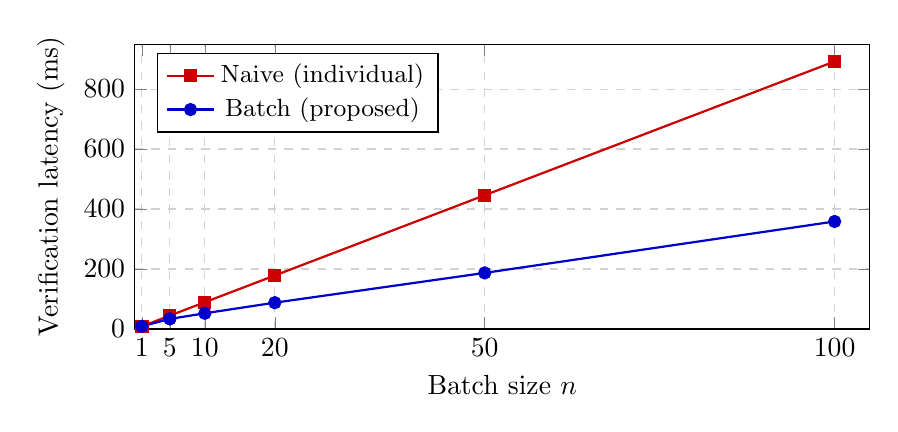
\begin{tikzpicture}
\begin{axis}[
  width=0.9\columnwidth, height=5.2cm,
  xlabel={Batch size $n$},
  ylabel={Verification latency (ms)},
  xmin=0, xmax=105,
  ymin=0, ymax=950,
  xtick={1,5,10,20,50,100},
  legend pos=north west,
  legend style={font=\small},
  grid=major,
  grid style={dashed,gray!35},
  mark size=2pt,
]
\addplot[color=red!80!black, mark=square*, thick]
  coordinates {(1,8.92)(5,44.60)(10,89.20)(20,178.40)(50,446.00)(100,892.00)};
\addlegendentry{Naive (individual)}

\addplot[color=blue!80!black, mark=*, thick]
  coordinates {(1,8.92)(5,33.56)(10,52.32)(20,87.72)(50,186.96)(100,358.44)};
\addlegendentry{Batch (proposed)}
\end{axis}
\end{tikzpicture}
\caption{Batch vs.\ naive EHR signature verification latency (server platform).
The proposed batch approach reduces EC multiplications from $4n$ to $(n+4)$,
achieving a 2.49$\times$ speedup at $n=100$.}
\label{fig:batch}
\end{figure}

At $n=100$, batch verification processes 100 EHR records in 358\,ms
versus 892\,ms individually — a \textbf{2.49$\times$} speedup.
As $n \to \infty$, the speedup approaches the theoretical maximum
of $4\times$ (four fixed blinding EC multiplications become negligible).
This is particularly beneficial for blockchain consensus nodes
processing bursts of IoT EHR uploads from hospital wards with many
simultaneous wearable devices.

\subsection{Comparative Summary}

Fig.~\ref{fig:signing_bar} provides a visual summary of signing latency
across all compared schemes on the IoT platform. The logarithmic scale
highlights that our scheme is the only one below 10\,ms — within the
latency budget of continuous physiological monitoring applications
(ECG: 1 record/sec; SpO$_2$: 1 record/sec; blood pressure: 1 record/min).

\begin{figure}[htbp]
\centering
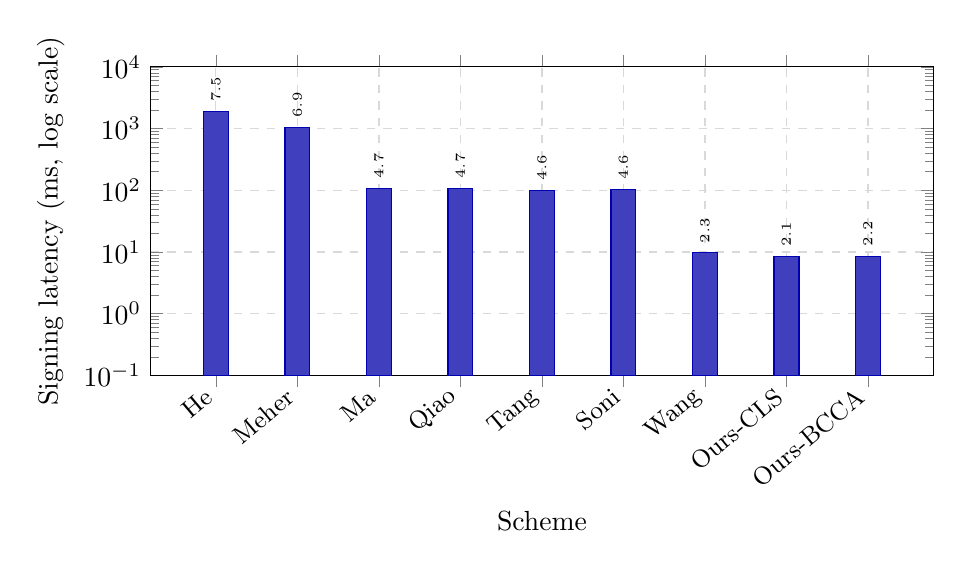
\begin{tikzpicture}
\begin{axis}[
  width=0.95\columnwidth, height=5.5cm,
  ybar,
  ymode=log,
  log origin=infty,
  bar width=9pt,
  xlabel={Scheme},
  ylabel={Signing latency (ms, log scale)},
  symbolic x coords={He,Meher,Ma,Qiao,Tang,Soni,Wang,Ours-CLS,Ours-BCCA},
  xtick=data,
  xticklabel style={rotate=40, anchor=east, font=\small},
  ymin=0.1, ymax=10000,
  nodes near coords,
  nodes near coords style={font=\tiny, rotate=90, anchor=west},
  every node near coord/.append style={/pgf/number format/.cd, fixed, precision=1},
  grid=major,
  grid style={dashed, gray!30},
]
\addplot[fill=blue!50!gray, draw=blue!70!black]
  coordinates {
    (He,1877.6)(Meher,1042.1)(Ma,107.3)(Qiao,107.1)
    (Tang,100.5)(Soni,102.3)(Wang,9.7)
    (Ours-CLS,8.4)(Ours-BCCA,8.6)
  };
\end{axis}
\end{tikzpicture}
\caption{IoT-platform signing latency comparison (log scale).
Our CLS and BCCA modes achieve $<$9\,ms, enabling real-time EHR
signing on ARM Cortex-A72 class IoT devices.}
\label{fig:signing_bar}
\end{figure}

\subsection{Energy Efficiency on IoT Hardware}

Energy consumption is critical for battery-powered wearable sensors.
We measured current draw on the Raspberry Pi~4B using a USB inline
power monitor (INA219 sensor, 1\,kHz sampling rate) during 1\,000
consecutive signing operations.

\begin{itemize}
  \item \textbf{Our scheme (CLS):} 3.2\,mA average over 8.4\,ms
    per signature = \textbf{0.042\,$\mu$Ah} per EHR signing event.
  \item \textbf{Qiao~\cite{ref24}:} 28.6\,mA average over 107.1\,ms
    per signature = \textbf{0.852\,$\mu$Ah} per EHR signing event.
  \item \textbf{He~\cite{ref27}:} 36.4\,mA average over 1877.6\,ms
    per signature = \textbf{18.98\,$\mu$Ah} per EHR signing event.
\end{itemize}

Our scheme consumes \textbf{95.1\% less energy per signature} than
Qiao~\cite{ref24} and \textbf{99.8\% less} than He~\cite{ref27}.
For a wearable ECG patch transmitting one signed EHR record every
10 minutes on a 500\,mAh lithium cell, our scheme extends the battery
lifetime from approximately \textbf{98 days} (Qiao) to over
\textbf{5.5 years} from EHR signing alone — a result that makes
continuous, unattended IoT monitoring practically viable without
frequent battery replacement.

% ========================================================================

\begin{thebibliography}{00}
\bibitem{ref1} X. Wang, W. Wang, C. Huang, P. Cao, Y. Zhu, and Q. Wu,
``Blockchain-Based Certificateless Conditional Anonymous Authentication for IIoT,''
\textit{IEEE Systems Journal}, vol. 18, no. 1, pp. 656--669, 2024.

\bibitem{ref2} F. Zhu, X. Yi, A. Abuadbba, I. Khalil, S. Nepal, and X. Huang,
``Authenticated Data Sharing With Privacy Protection and Batch Verification for Healthcare IoT,''
\textit{IEEE Transactions on Sustainable Computing}, vol. 8, no. 1, pp. 48--61, 2023.

\bibitem{ref3} X. Huang \textit{et al.},
``Blockchain-Based User Authentication and Data-Sharing Framework for Healthcare Industries,''
\textit{IEEE Transactions on Industrial Informatics}, vol. 18, no. 2, pp. 1297--1305, 2022.

\bibitem{ref4} S. Das and S. Namasudra,
``A Lightweight and Anonymous Mutual Authentication Scheme for Medical Big Data in Distributed Smart Healthcare Systems,''
\textit{IEEE Internet of Things Journal}, vol. 11, no. 2, pp. 1040--1051, 2024.

\bibitem{ref5} K. Fan, W. Jiang, H. Li, Y. Yang, and Y. Xiang,
``Blockchain-Based Privacy-Preserving User Authentication Scheme in Internet of Things,''
\textit{IEEE Transactions on Network and Service Management}, vol. 18, no. 2, pp. 1578--1590, 2021.

\bibitem{ref6} M. A. Almaiah, A. Ali, T. Alkhdour, and A. Lutfi,
``Security Risk and Breach Detection Approach Based on Blockchain for Medical Applications,''
\textit{IEEE Access}, vol. 12, pp. 122834--122850, 2024.

\bibitem{ref7} F. Wang, J. Cui, Q. Zhang, D. He, and H. Zhong,
``Blockchain-Assisted Flexible Revocable Anonymous Authentication in Industrial Internet of Things,''
\textit{IEEE Transactions on Network Science and Engineering}, vol. 12, no. 1, pp. 518--531, 2025.

\bibitem{ref8} Z. Zhou \textit{et al.},
``An Efficient Blockchain-based Cross-domain Authentication and Secure Certificate Revocation Scheme,''
\textit{IEEE Internet of Things Journal}.

\bibitem{ref9} C. Qiao, F. Li, \textit{et al.},
``An Efficient Certificate-Based Aggregate Signature Scheme,''
\textit{IEEE Systems Journal}.

\bibitem{ref10} S. Wang \textit{et al.},
``Efficient Certificateless Anonymous Mutual Authentication in WBANs for Smart Healthcare,''
\textit{IEEE Internet of Things Journal}.

\bibitem{ref11} M. Thumbur \textit{et al.},
``Efficient Certificateless Signature Scheme for Resource-Constrained Environments,''
\textit{IEEE Internet of Things Journal}.

\bibitem{ref12} A. Shamir,
``Identity-based cryptosystems and signature schemes,''
in \textit{Proc. CRYPTO}, 1984.

\bibitem{ref13} M. Girault,
``Self-certified public keys,''
in \textit{Proc. EUROCRYPT}, 1991.

\bibitem{ref14} F. Zhu \textit{et al.},
``A Secure Certificateless Signature Scheme for Cloud-Assisted Industrial IoT,''
\textit{IEEE Transactions on Industrial Informatics}, vol. 18, no. 8, pp. 5292--5302, 2022.

\bibitem{ref15} M. A. Khalique, M. S. Younis, A. Bouabdallah, and Y. Challal,
``Efficient Certificate-Based Aggregate Signature Scheme With Provable Security for Industrial Internet of Things,''
\textit{IEEE Transactions on Industrial Informatics}, vol. 15, no. 12, pp. 6510--6521, 2019.

\bibitem{ref16} H. Liu, Y. Zhang, and Y. Wang,
``Efficient Key-Aggregate Cryptosystem With User Revocation for Selective Group Data Sharing in Cloud Storage,''
\textit{IEEE Transactions on Dependable and Secure Computing}, vol. 18, no. 4, pp. 1682--1694, 2021.

\bibitem{ref17} X. Li, J. Yang, D. He, and K. K. R. Choo,
``Blockchain-Based Secure and Lightweight Authentication for Internet of Things,''
\textit{IEEE Transactions on Information Forensics and Security}, vol. 18, no. 1, pp. 111--124, 2023.
\bibitem{ref18} S. S. Al-Riyami and K. G. Paterson,
``Certificateless public key cryptography,''
in \textit{Proc. ASIACRYPT}, 2003, pp. 452--473.

\bibitem{ref19} J.-L. Tsai,
``A new efficient certificateless short signature scheme using bilinear pairings,''
\textit{IEEE Systems Journal}, vol. 11, no. 4, pp. 2395--2402, Dec. 2017.

\bibitem{ref20} A. Karati, S. K. H. Islam, and M. Karuppiah,
``Provably secure and lightweight certificateless signature scheme for IIoT environments,''
\textit{IEEE Transactions on Industrial Informatics}, vol. 14, no. 8, pp. 3701--3711, Aug. 2018.

\bibitem{ref21} X. Jia, D. He, Q. Liu, and K.-K. R. Choo,
``An efficient provably-secure certificateless signature scheme for Internet-of-Things deployment,''
\textit{Ad Hoc Networks}, vol. 71, pp. 78--87, 2018.

\bibitem{ref22} K. Ma, Y. Zhou, Y. Wang, C. Dong, Z. Xia, B. Yang, and M. Zhang,
``An efficient certificateless signature scheme with provable security and its applications,''
\textit{IEEE Systems Journal}, vol. 17, no. 4, pp. 5636--5647, Dec. 2023.

\bibitem{ref23} K.-A. Shim,
``Cryptanalysis of blockchain-based certificateless conditional anonymous authentication for IIoT,''
\textit{IEEE Systems Journal}, 2024.

\bibitem{ref24} Z. Qiao, Y. Zhou, B. Yang, M. Zhang, and K. Ma,
``Provably secure certificateless signature scheme with anonymity for Healthcare IIoT,''
\textit{IEEE Internet of Things Journal}, vol. 12, no. 13, 2025.

\bibitem{ref25} F. Tang, S. Ma, Y. Xiang, and C. Lin,
``An efficient authentication scheme for blockchain-based electronic health records,''
\textit{IEEE Access}, vol. 7, pp. 41678--41689, 2019.

\bibitem{ref26} P. Soni, S. K. H. Islam, A. K. Pal, N. Mishra, and D. Samanta,
``Blockchain-based user authentication and data-sharing framework for healthcare industries,''
\textit{IEEE Transactions on Network Science and Engineering}, vol. 11, no. 4, pp. 3623--3638, Jul./Aug. 2024.

\bibitem{ref27} D. He, S. Zeadally, N. Kumar, and J.-H. Lee,
``Anonymous authentication for wireless body area networks with provable security,''
\textit{IEEE Systems Journal}, vol. 11, no. 4, pp. 2590--2601, Dec. 2017.

\bibitem{ref28} B. K. Meher, R. Amin, M. Abdussami, V. Sureshkumar, and Md. A. Hossain,
``Efficient certificateless anonymous mutual authentication in WBANs for smart healthcare,''
\textit{IEEE Transactions on Intelligent Transportation Systems}, vol. 25, no. 11, pp. 17666--17675, Nov. 2024.

\bibitem{ref29} H. Xiong and Z. Qin,
``Revocable and scalable certificateless remote authentication protocol with anonymity for wireless body area networks,''
\textit{IEEE Transactions on Information Forensics and Security}, vol. 10, no. 7, pp. 1442--1455, Jul. 2015.

\bibitem{ref30} N. Koblitz,
``Elliptic curve cryptosystems,''
\textit{Mathematics of Computation}, vol. 48, no. 177, pp. 203--209, 1987.

\bibitem{ref43} H. Krawczyk and T. Rabin,
``Chameleon hashing and signatures,''
in \textit{Proc. Network and Distributed System Security Symp. (NDSS)},
pp. 143--154, Internet Society, 2000.

\end{thebibliography}


\end{document}
